\documentclass{standalone}
\usepackage{pgfplots}
\pgfplotsset{compat=1.17}

\begin{document}

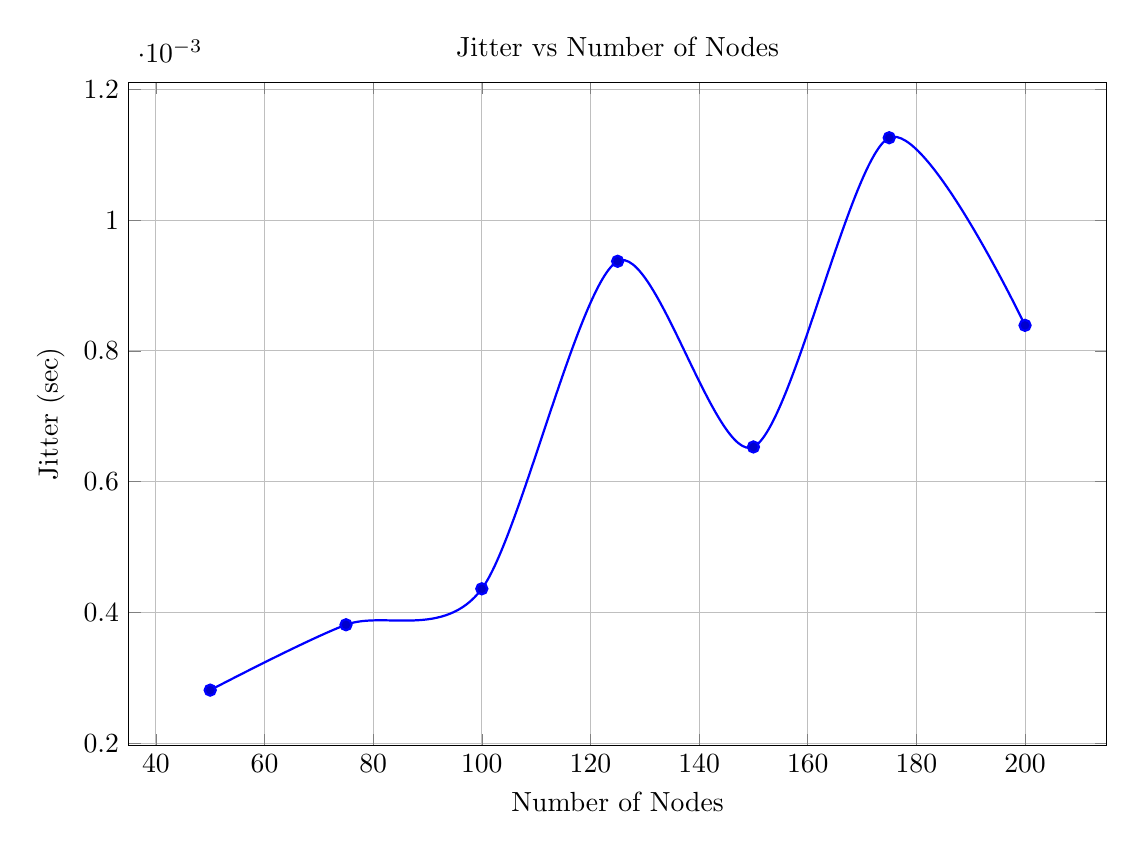
\begin{tikzpicture}
\begin{axis}[
width=14cm,height=10cm,
title={Jitter vs Number of Nodes},
xlabel={Number of Nodes},
ylabel={Jitter (sec)},
grid=major]

\addplot+[smooth,mark=*,thick] coordinates {
(50,0.000281)(75,0.000381)(100,0.000436)
(125,0.000937)(150,0.000653)(175,0.001126)(200,0.000839)
};

\end{axis}
\end{tikzpicture}

\end{document}